\documentclass{article}
\usepackage{amsmath}
\usepackage{mathtools}
\usepackage[margin=1in]{geometry}
\usepackage{hyperref}
\usepackage{amsfonts}
\hypersetup{colorlinks,urlcolor=blue}

\title{Problem 126}
\author{https://github.com/self-gautrang}
\date{April 2020}

\begin{document}

\maketitle

\section{Question}
\href{https://projecteuler.net/problem=126}{https://projecteuler.net/problem=126}.

\section{Number of blocks of a cuboid being covered by $n$ layers}
\indent Assume we have a cuboid of size a\texttt{x}b\texttt{x}c. 
Suppose, for example, $a=3$, $b=1$, $c=3$.  
It is challenging to visualize filling the cuboid in a 3D coordinate system, especially for $n \geq 2$. 
To address this, we take the cross sections of the cuboid along one coordinate. 
In the figure below, we split the cuboid to 3 pieces of size $3 \texttt{x} 1$. \\
\begin{figure}[h]
  \centering
    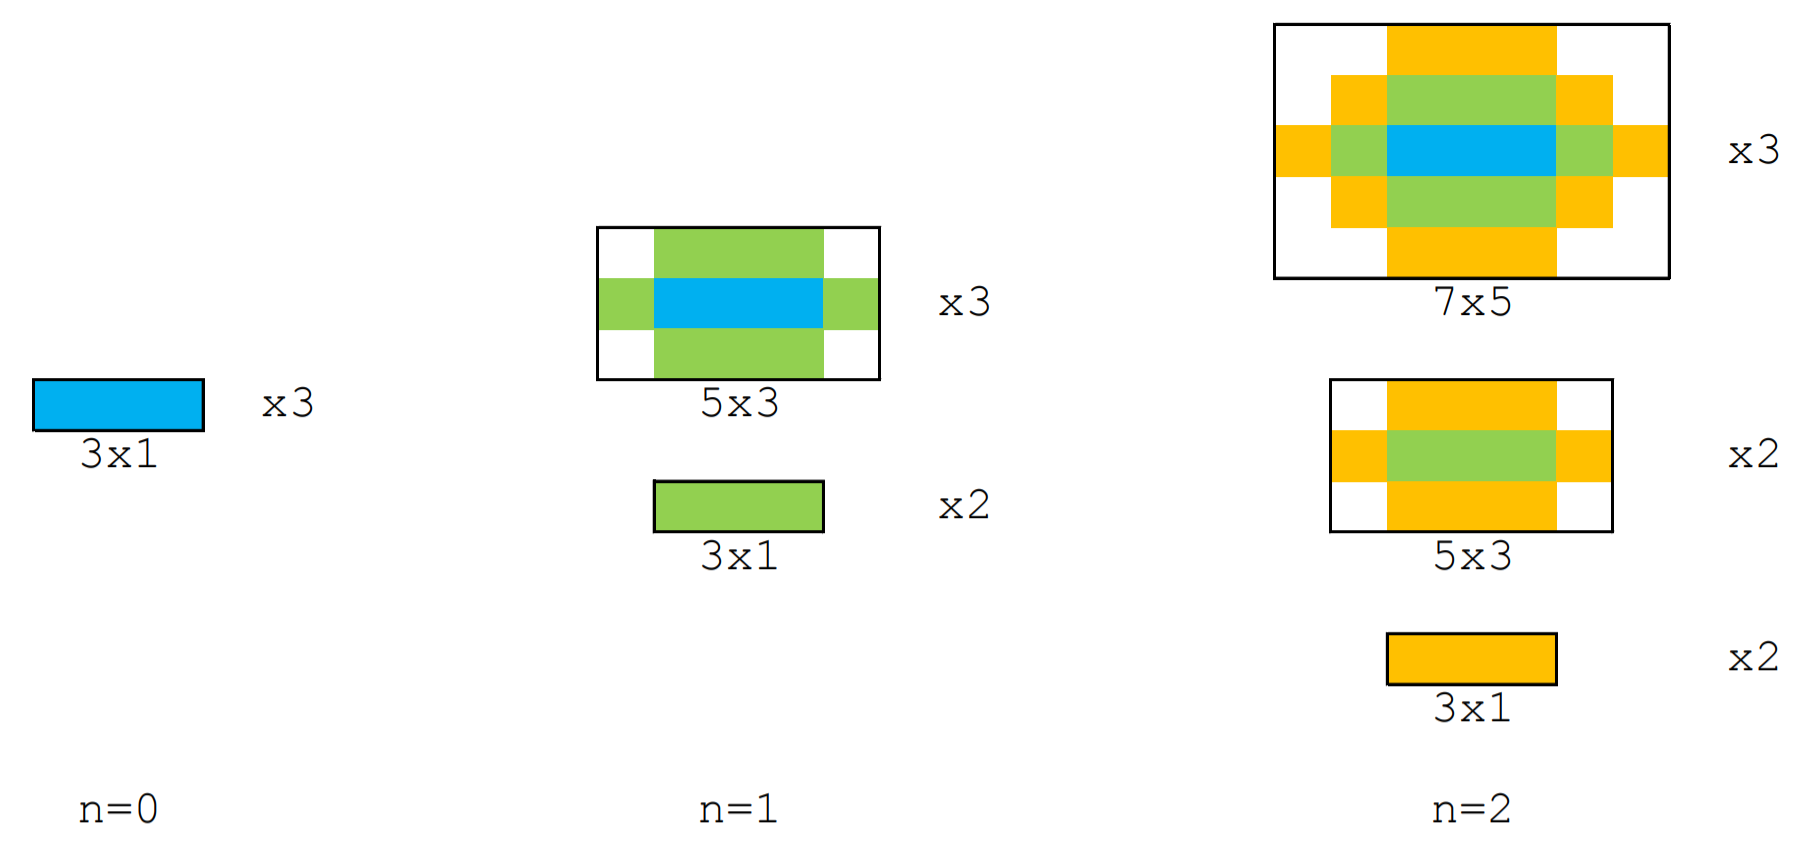
\includegraphics[width=0.75\textwidth]{images/p126_1.png}
  \caption{At $n=0$, we have the original $3\texttt{x}1\texttt{x}3$ cuboid being split to 3 pieces of size $3 \texttt{x} 1$. 
  At $n=1$, for each $3 \texttt{x} 1$ of $n = 0$, we need to cover all of their 4 sides. 
  Other than that, we also need to cover the front of the most outer $3 \texttt{x} 1$ of $n = 0$ that facing out of the paper, and to cover the back of the most inner $3 \texttt{x} 1$ of $n = 0$ that facing towards the paper. 
  The newly add pieces are illustrated by the green blocks, while the original pieces are the blue blocks. 
  At $n=2$, we need to cover the green blocks exposing the white blocks. 
  The strategy of covering $n=1$ is the same as what we do to cover $n=0$. 
  The newly add pieces are illustrated by the orange blocks.}
\end{figure}\\
\indent From the observations above, we have that, a block of size $a\texttt{x}b$ grows to $(a+2) \texttt{x} (b+2)$ minus $4 \times 1$ white blocks, which turns to $(a+4) \texttt{x} (b+4)$ minus $4 \times (1+2)$ white blocks in the next iteration. 
In general, in the $k^{th}$ iteration, the original tiles of size $a \texttt{x} b$ will turn into $(a+2k)(b+2k)-4\sum_{i=0}^{k}i$, or $(a+2k)(b+2k)-2k(k+1)$. 
Another observation is that, each iteration will add two new $a\texttt{x}b$ blocks, while other blocks grow. \\
\indent Let $f(a,b,c,n) \rightarrow \mathbb{N}$ be a function that calculates the number of blocks of a cuboid of size $a\texttt{x}b\texttt{x}c$ being covered by $n$ layers.
\begin{align*}
    f(a,b,c,n) &= c[(a+2n)(b+2n) - 2n(n+1)] + 2\sum_{i=0}^{n-1}[(a+2i)(b+2i)-2i(i+1)]
\end{align*}
as at iteration $n$, we have $c$ cross-sections grow from the original cuboid, as other 2 per iteration.
\section{Number of blocks needed to transform a cuboid of $n-1$ layers into $n$ layers}
\indent Let $g(a,b,c,n) \rightarrow \mathbb{N}$ be a function that calculates the number of blocks needed to transform a cuboid of size $a\texttt{x}b\texttt{x}c$ being covered by $n-1$ layers into the one covered by $n$ layers.
\begin{align*}
    g(a,b,c,n) &=f(a,b,c,n) - f(a,b,c,n-1)\\
    &=c(a+2n)(b+2n)-c(a+2n-2)(b+2n-2) \\
    & \texttt{\thinspace\thinspace\thinspace\thinspace\thinspace}- 2cn(n+1) + 2c(n-1)n + 2(a+2n-2)(b+2n-2)-4(n-1)n \\
    &=2ab + 2ac + 4an - 4a + 2bc + 4bn - 4b + 4cn - 4c + 4n^2 - 12 n + 8\\
    &=2(ab+ac+bc)+4(n-1)(a+b+c)+4(n-1)(n-2)
\end{align*}

\end{document}

